\documentclass[a4paper,fleqn]{cas-sc}
% High-level Commands
\newcommand{\version}{v1/}
\newcommand{\eg}{\textit{e.g.}}

% Math Commands
\newcommand{\dispx}{u_{x_{1:t}}}
\newcommand{\dispy}{u_{y_{1:t}}}
\newcommand{\avgstress}{\bar{\sigma}_{1:t}}
\newcommand{\avgstrain}{\bar{\epsilon}_{1:t}}

\usepackage[authoryear,longnamesfirst]{natbib}
\usepackage{subcaption}
%\RequirePackage{cas-common}

%%%Author macros
\def\tsc#1{\csdef{#1}{\textsc{\lowercase{#1}}\xspace}}
\tsc{WGM}
\tsc{QE}

% Uncomment and use as if needed
%\newtheorem{theorem}{Theorem}
%\newtheorem{lemma}[theorem]{Lemma}
%\newdefinition{rmk}{Remark}
%\newproof{pf}{Proof}
%\newproof{pot}{Proof of Theorem \ref{thm}}

\begin{document}
\let\WriteBookmarks\relax
\def\floatpagepagefraction{1}
\def\textpagefraction{.001}

% Short title
\shorttitle{Cooperative Data-driven Modeling}    

% Short author
%\shortauthors{<short author list for running head>}  

% Main title of the paper
\title[mode=title]{Cooperative Data-driven Modeling}  

% Title footnote mark
% eg: \tnotemark[1]
%\tnotemark[1] 

% Title footnote 1.
% eg: \tnotetext[1]{Title footnote text}
%\tnotetext[1]{Title footnote text} 

% First author
%
% Options: Use if required
% eg: \author[1,3]{Author Name}[type=editor,
%       style=chinese,
%       auid=000,
%       bioid=1,
%       prefix=Sir,
%       orcid=0000-0000-0000-0000,
%       facebook=<facebook id>,
%       twitter=<twitter id>,
%       linkedin=<linkedin id>,
%       gplus=<gplus id>]

\author[1]{A}

% Corresponding author indication

% Footnote of the first author
%\fnmark[<footnote mark no>]

% Email id of the first author
%\ead{<email address>}

% URL of the first author
%\ead[url]{<URL>}

% Credit authorship
% eg: \credit{Conceptualization of this study, Methodology, Software}
%\credit{<Credit authorship details>}

% Address/affiliation
\affiliation[1]{organization={Delft University of Technology},
            addressline={}, 
            city={},
%          citysep={}, % Uncomment if no comma needed between city and postcode
            postcode={}, 
            state={},
            country={}}


\author[2]{B}
% Footnote of the second author
%\fnmark[2]

% Email id of the second author
%\ead{}

% URL of the second author
%\ead[url]{}

% Credit authorship
%\credit{}

% Address/affiliation
\affiliation[2]{organization={Delft University of Technology},
            addressline={}, 
            city={},
%          citysep={}, % Uncomment if no comma needed between city and postcode
            postcode={}, 
            state={},
            country={}}



\author[3]{C}
% Footnote of the third author
%\fnmark[3]

%Email id of the third author
\ead{miguel_bessa@brown.edu}

% URL of the third author
%\ead[url]{}

% Credit authorship
%\credit{}

% Address/affiliation
\affiliation[3]{organization={Brown University},
            addressline={}, 
            city={},
%          citysep={}, % Uncomment if no comma needed between city and postcode
            postcode={}, 
            state={},
            country={}}

\cormark[1]
\cortext[1]{Corresponding author}

% Footnote text
%\fntext[3]{}

% For a title note without a number/mark
%\nonumnote{}

% Here goes the abstract
\begin{abstract}
Abstract
\end{abstract}

% Use if graphical abstract is present
%\begin{graphicalabstract}
%\includegraphics{}
%\end{graphicalabstract}

% Research highlights
\begin{highlights}
\item 
\item 
\item 
\end{highlights}

% Keywords
% Each keyword is seperated by \sep
\begin{keywords}
 \sep data-driven modeling \sep continual learning \sep transfer learning \sep plasticity
\end{keywords}

\maketitle

% Numbered list
% Use the style of numbering in square brackets.
% If nothing is used, default style will be taken.
%\begin{enumerate}[a)]
%\item 
%\item 
%\item 
%\end{enumerate}  

% Unnumbered list
%\begin{itemize}
%\item 
%\item 
%\item 
%\end{itemize}  

% Description list
%\begin{description}
%\item[]
%\item[] 
%\item[] 
%\end{description}  

% Figure
%\begin{figure}[<options>]
%	\centering
%		\includegraphics[<options>]{}
%	  \caption{}\label{fig1}
%\end{figure}


%\begin{table}[<options>]
%\caption{}\label{tbl1}
%\begin{tabular*}{\tblwidth}{@{}LL@{}}
%\toprule
%  &  \\ % Table header row
%\midrule
% & \\
% & \\
% & \\
% & \\
%\bottomrule
%\end{tabular*}
%\end{table}

% Main text
\section{Introduction}\label{sec:intro}
  % Mechanics and computational power
The mechanics followed a deterministic approach for many years. This deterministic approaches helped humanity in various engineering and design problems. Over the last 5 decades engineering problems got increasingly complexer as the needs of the humanity changed in a similar fashion. These complex problems are tackled mostly with the combination of experimental and computer aided simulations until recently. In this combined endeavour, where experiments are hindered, computer aided simulations helped significantly eliminate the money and time limitations of the experimental approach. Especially due to increasing availability and accessibility of the computational power. Although, their wide spread use the deterministic high-fidelity numerical solutions, also known as computer aided simulations, requirement of time and money is also increasing as the complexity of the problems increase further. It is getting evidently clear that the Moore's Law is loosing its validity due to physical limitations of the silicone technology \cite{arenas2021}. Thus, if we want to continue solving complex problems in the coming future, the need for another approach that can further reduce the time and money requirements of the current experimental and computer aided numerical solutions.

% ML in mechanics
Machine learning (ML) applications from computer-vision, to speech-recognition are getting more and more essential part of our daily life. To this end, it is not a surprise that ML found use cases in mechanics as well. To the authors knowledge the first mechanics applications of the machine learning paradigm dates back to the second-boom (1990's till 2000's) of ML in the fields of civil and mechanical engineering (\eg \cite{reich1997,reich1995,bishop1993,adeli}). Similar to numerical method applications used in the field of mechanics, machine learning also benefited from the increasing computational power. However, to reach the popularity and wide-spread application areas can be attributed to the more open and development aimed attitude of the field. This increasing open-access to ML tools the applied use cases of the ML in the mechanics community started to flourish.

% Recent landscape
The effort put into decrease the time complexity of the direct numerical solutions, is sprouting. On one hand a general way to tackle the differential equations resulting in a mechanics problem is being tackled. For instance,  Physics-Informed Neural Networks (PINNs) \cite{raissi2019b} and it variants, where the fields of interests are represented as neural networks and the residual enforced by the differential equations, and initial and boundary conditions are minimized.  Moreover, the operators that are the key parts of differential equations are tried to be learn from the data in \cite{lu2021a}. On the other hand, more specific applications try to tackle more specific sub-problems with the help of various ML techniques. These examples mostly try to accelerate a certain part of a certain problem via data-driven approaches. Due to its nested structure the time complexity of the multi-scale direct numerical solutions are one of the most laborious endeavours in solid mechanics espcially when coupled with other physical-phenomenon. In \cite{bessa2017} one such application is shown where a multi-scale problem is tried to be tackled in micro-scale. Due to data hungry ML applications, another type of ML application, which is ML based reduced order models (\qg \cite{liu2016,ferreira2021}), are utilized. The utilization of these data hungry applications 

One of the major application areas involve the multi-scale 


% Problems with the landscape


% How can we solve these problems?


% The aim of the paper?


% Landscape of the current literature wrt our aim! 






\section{Continual learning}\label{sec:cl}

\subsection{Methods overview}\label{subsec:overview}

\section{Proposed method (CDDM)}\label{sec:method}

\section{Numerical experiments}\label{sec:numerical_exp}
\subsection{Data generation}\label{subsec:data}
  % Problem explanation
In this paper, an elastoplastic von Mises material without hardening is investigated to create a path-dependent problem. A fixed-sized square is utilized as a domain and holes of varying sizes and orientations are placed inside the domain to create different tasks. The tasks originating from different domains can be seen in Figure \ref{fig:tasks}. For all the tasks bottom part of the domain is fixed and the top part is displaced in $\dispx$ and $\dispy$ to introduce deformation to the domain (see Figure \ref{fig:problem}). After, the displacement the average Cauchy strain ($\avgstrain$) and Cauchy stress ($\avgstress$) measures are obtained for the deformation path. Then the learning problem for the $i$-th task can be defined as,
\begin{equation}
  \avgstress = f_i(\avgstrain),
\end{equation}
where a machine learning model can be utilized the find the relationship $f_i:=\avgstrain \to \avgstress$. 

% Continual Learning Problem

% Data generation
In the described problem 1000 paths for 100 displacement values are sampled for the top boundary of the domain sampled from a Gaussian Process posterior that is conditioned on 20 displacement values sampled from a uniform distribution for each path. The resulting displacement paths are utilized to obtain average stress and strains. For each presented task the same deformation paths are utilized to calculate the domain-specific average stress and strain values. The data is generated using FEniCS \cite{logg2012a}. 

% Tasks 

%Difference between tasks (I think we should present the Figures that Aleksandr showed on the difference between the tasks here.




\begin{figure}
  \centering
  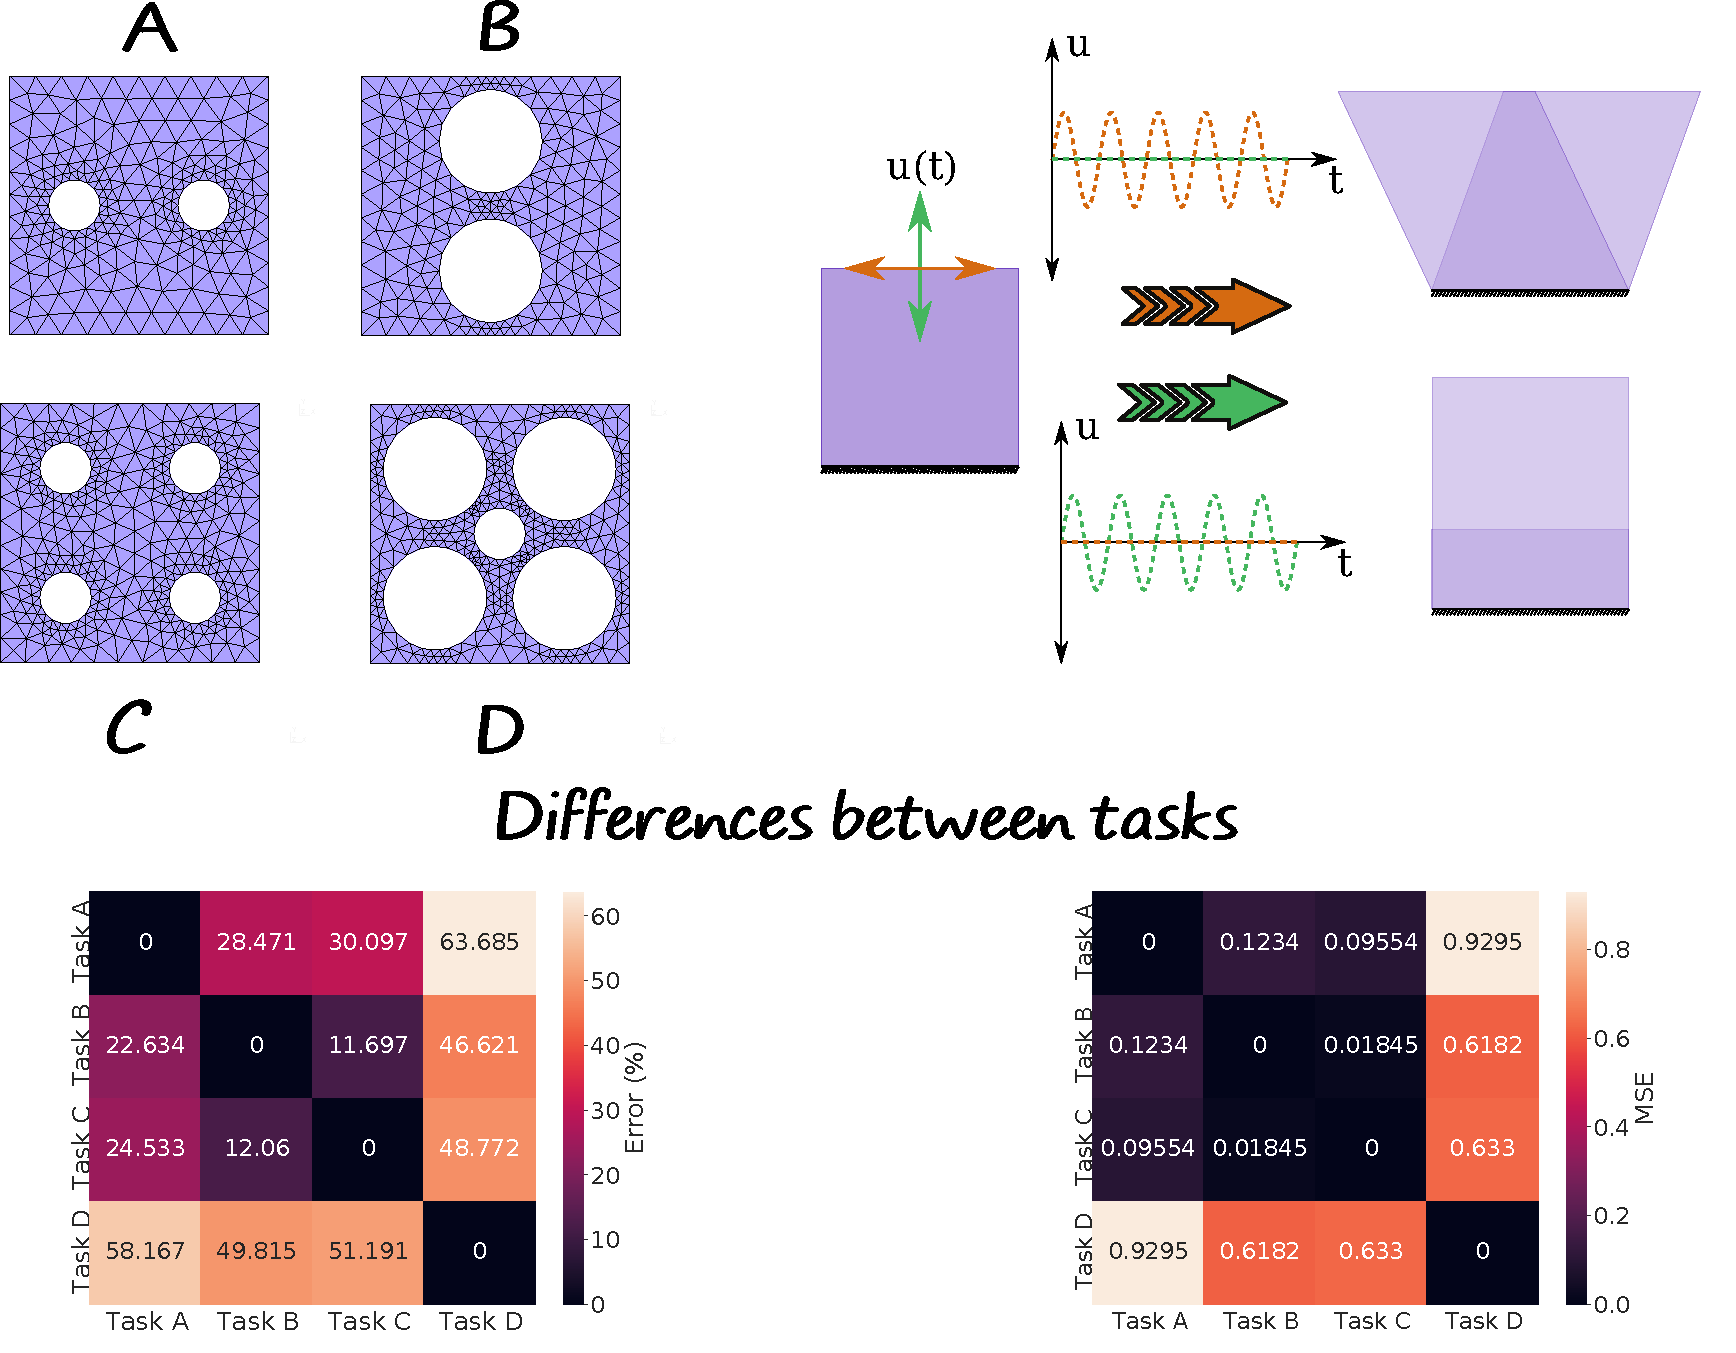
\includegraphics[scale=0.4]{Figures_\version/problem.pdf}
  \caption{A square domain with fixed on the bottom and displaced on the top. Displacement is done in a pseudo-time.}
  \label{fig:problem}
\end{figure}
\begin{figure}
  \centering
  \begin{subfigure}[b]{0.22\textwidth}
    \centering
    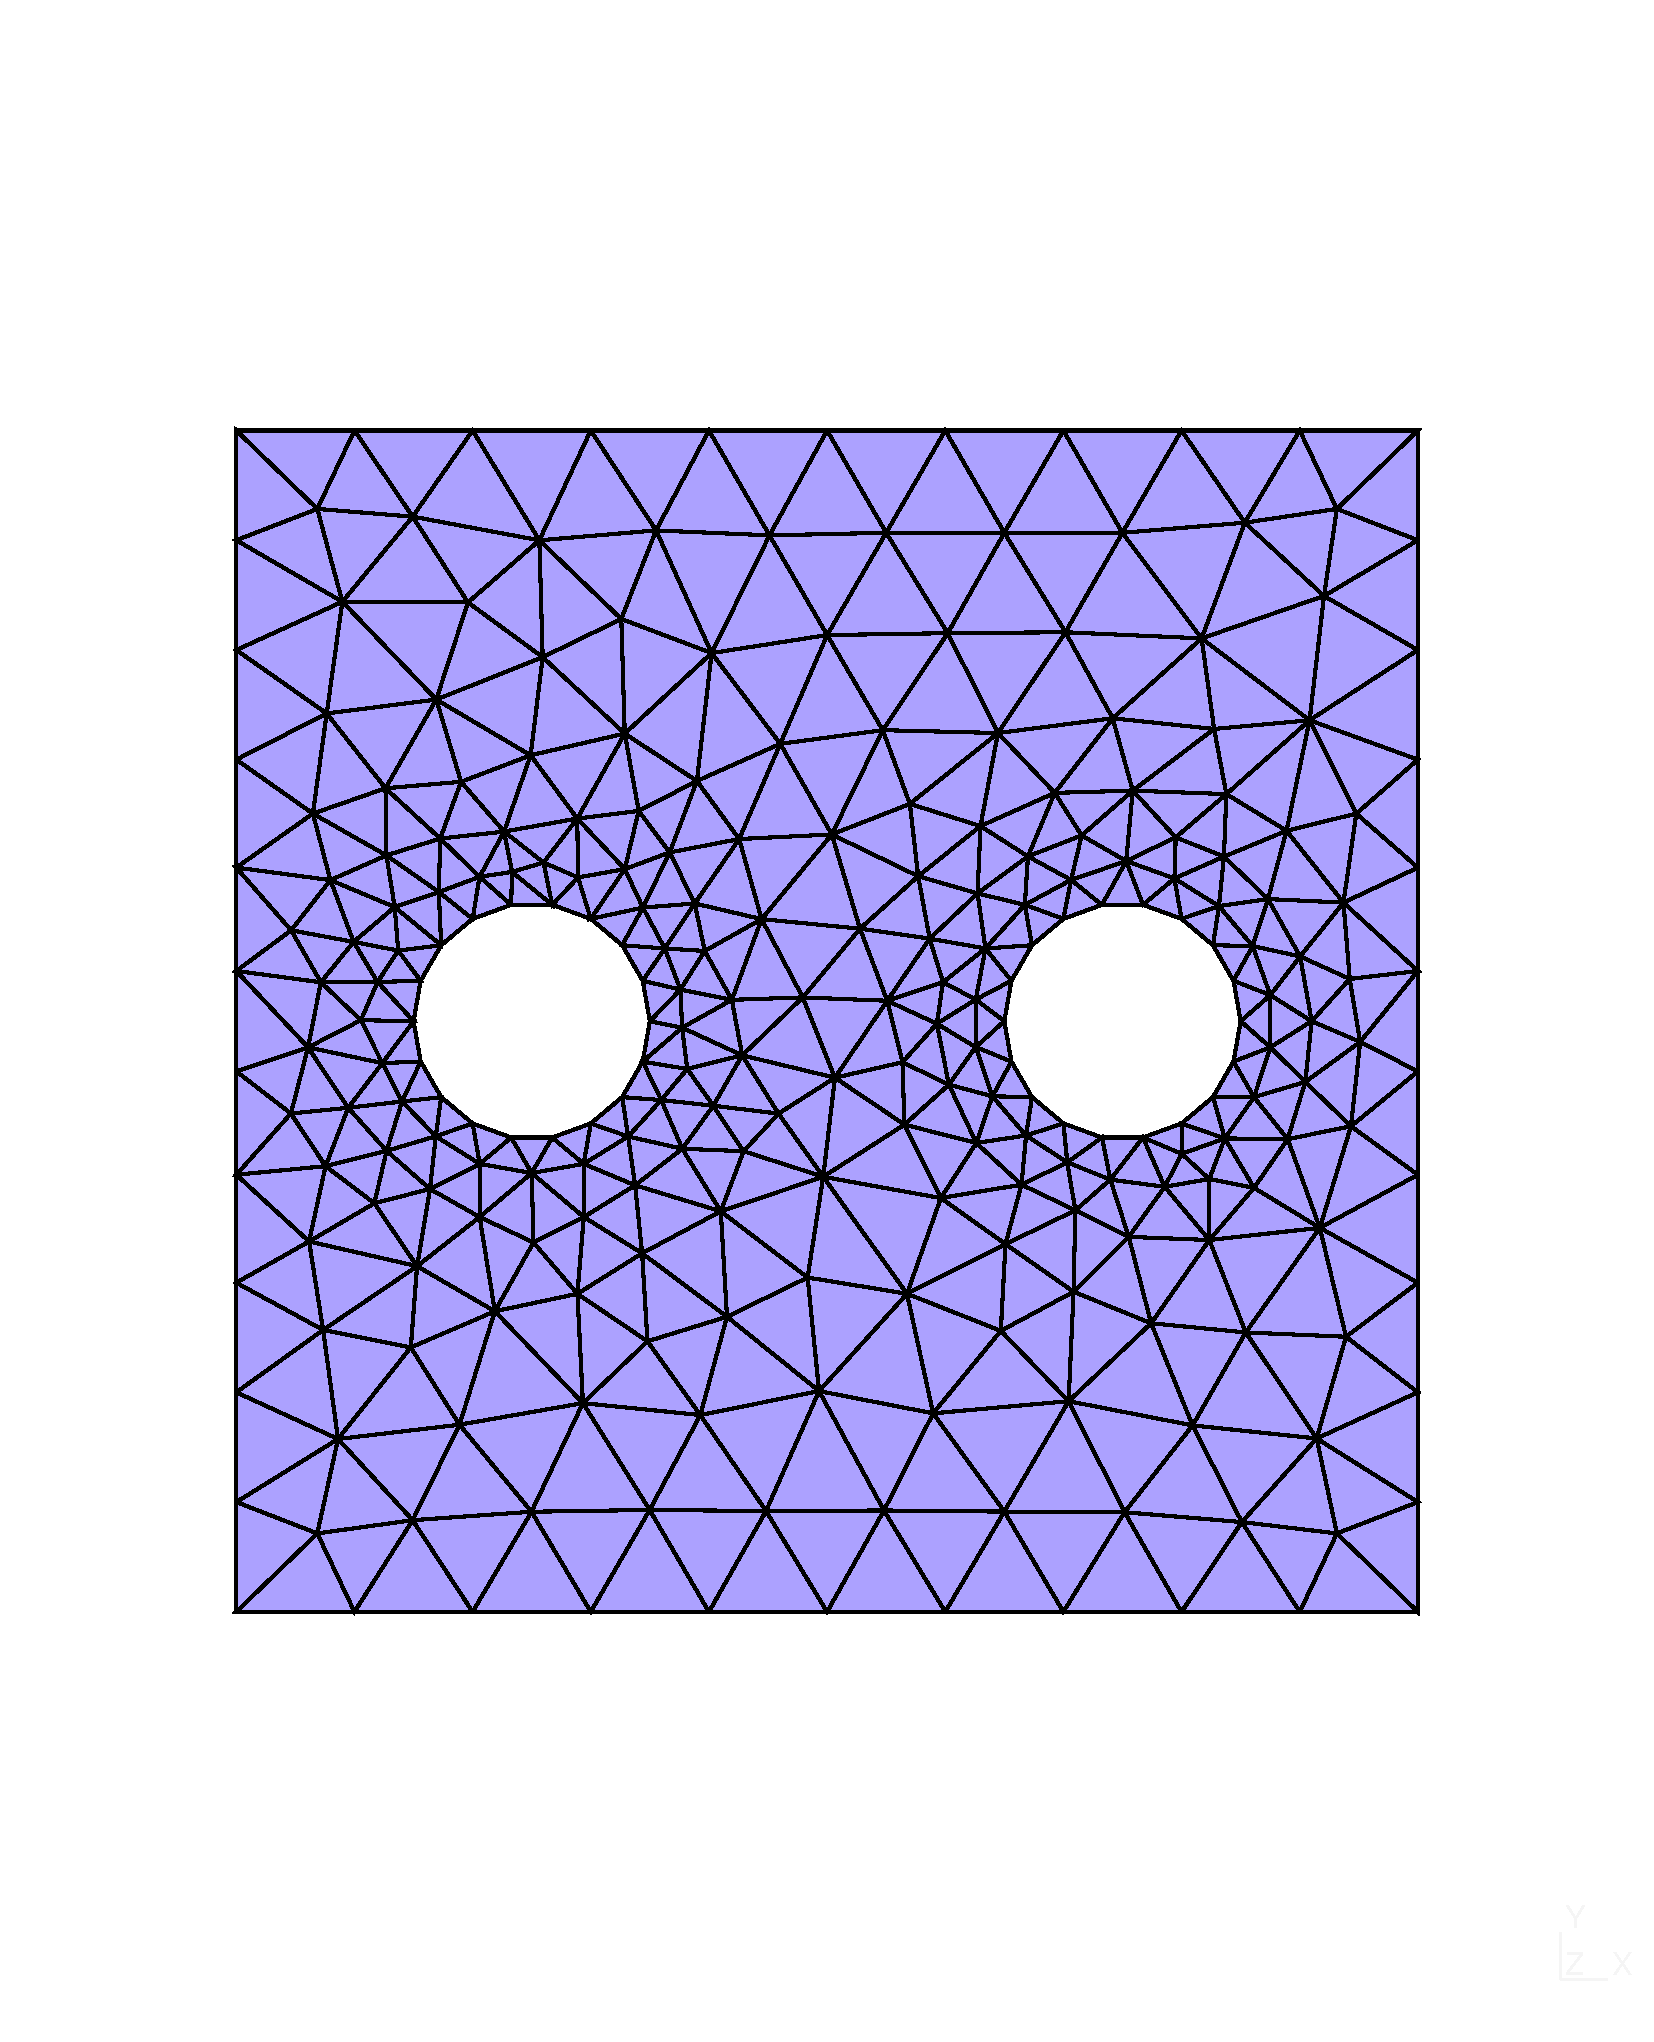
\includegraphics[width=\textwidth]{Figures_\version/tasks/2_on_x.pdf}
    \caption{Task 1}
    \label{fig:task1}
  \end{subfigure}
  \hfill
  \begin{subfigure}[b]{0.22\textwidth}
    \centering
    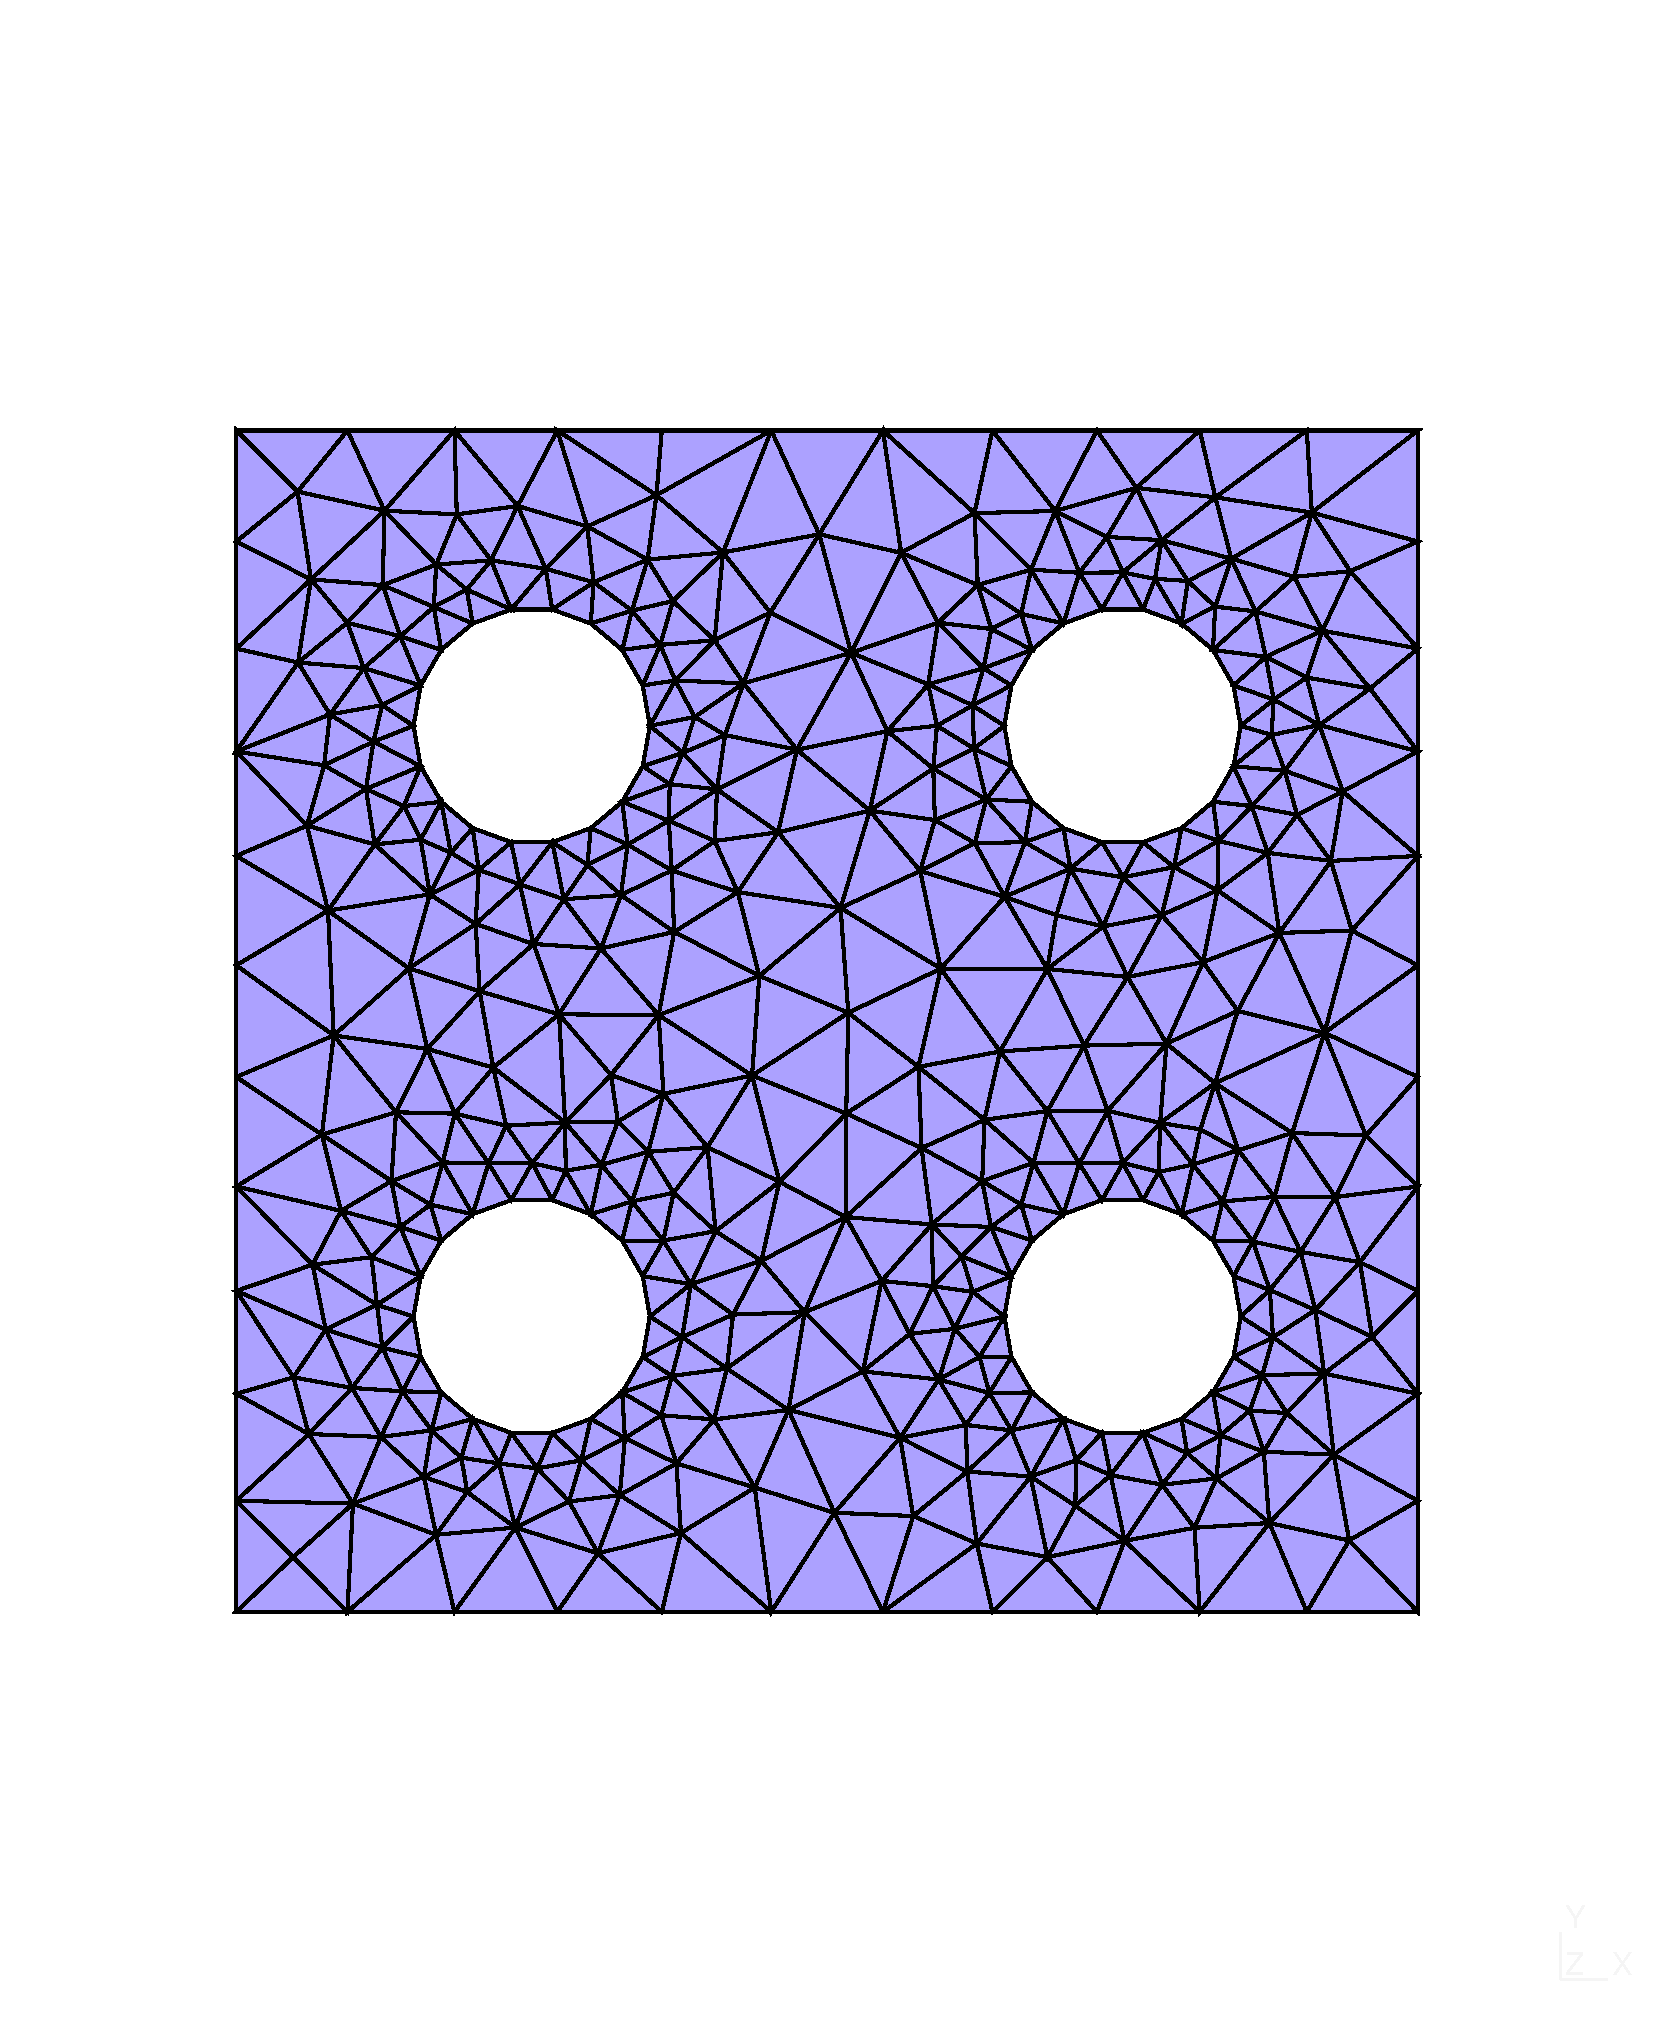
\includegraphics[width=\textwidth]{Figures_\version/tasks/4_diagonal.pdf}
    \caption{Task 2}
    \label{fig:task2}
  \end{subfigure}
  \hfill
  \begin{subfigure}[b]{0.22\textwidth}
    \centering
    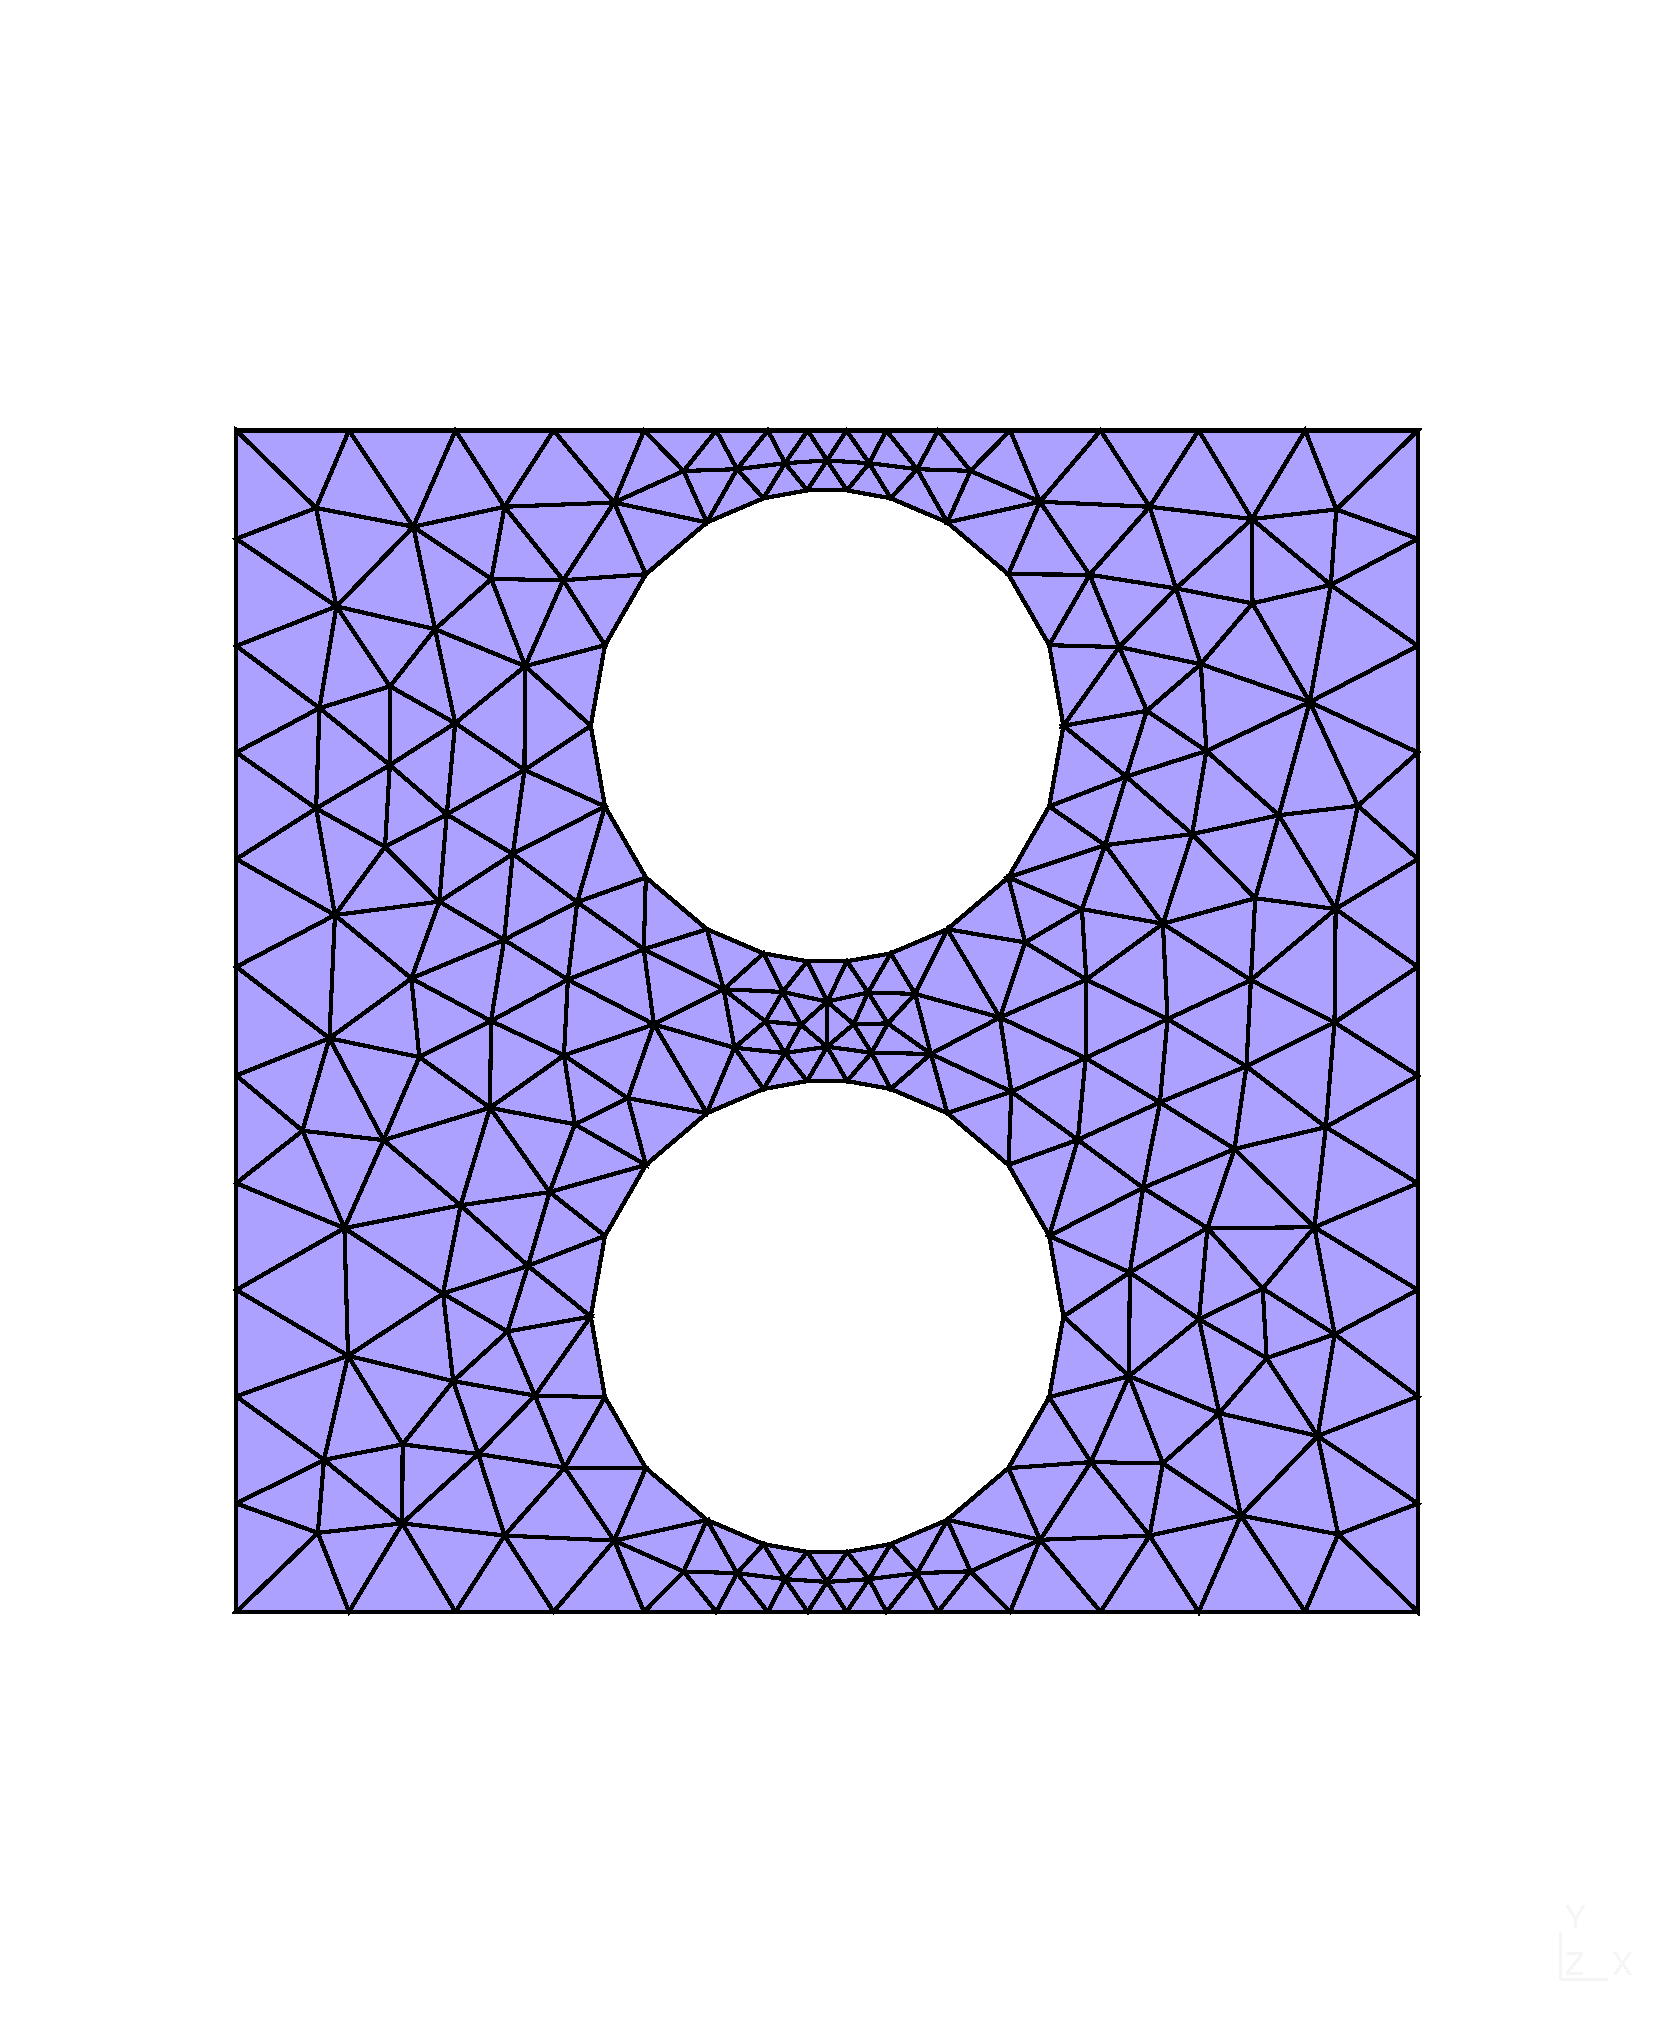
\includegraphics[width=\textwidth]{Figures_\version/tasks/2_on_y.pdf}
    \caption{Task 3}
    \label{fig:task3}
  \end{subfigure}
  \hfill
  \begin{subfigure}[b]{0.22\textwidth}
    \centering
    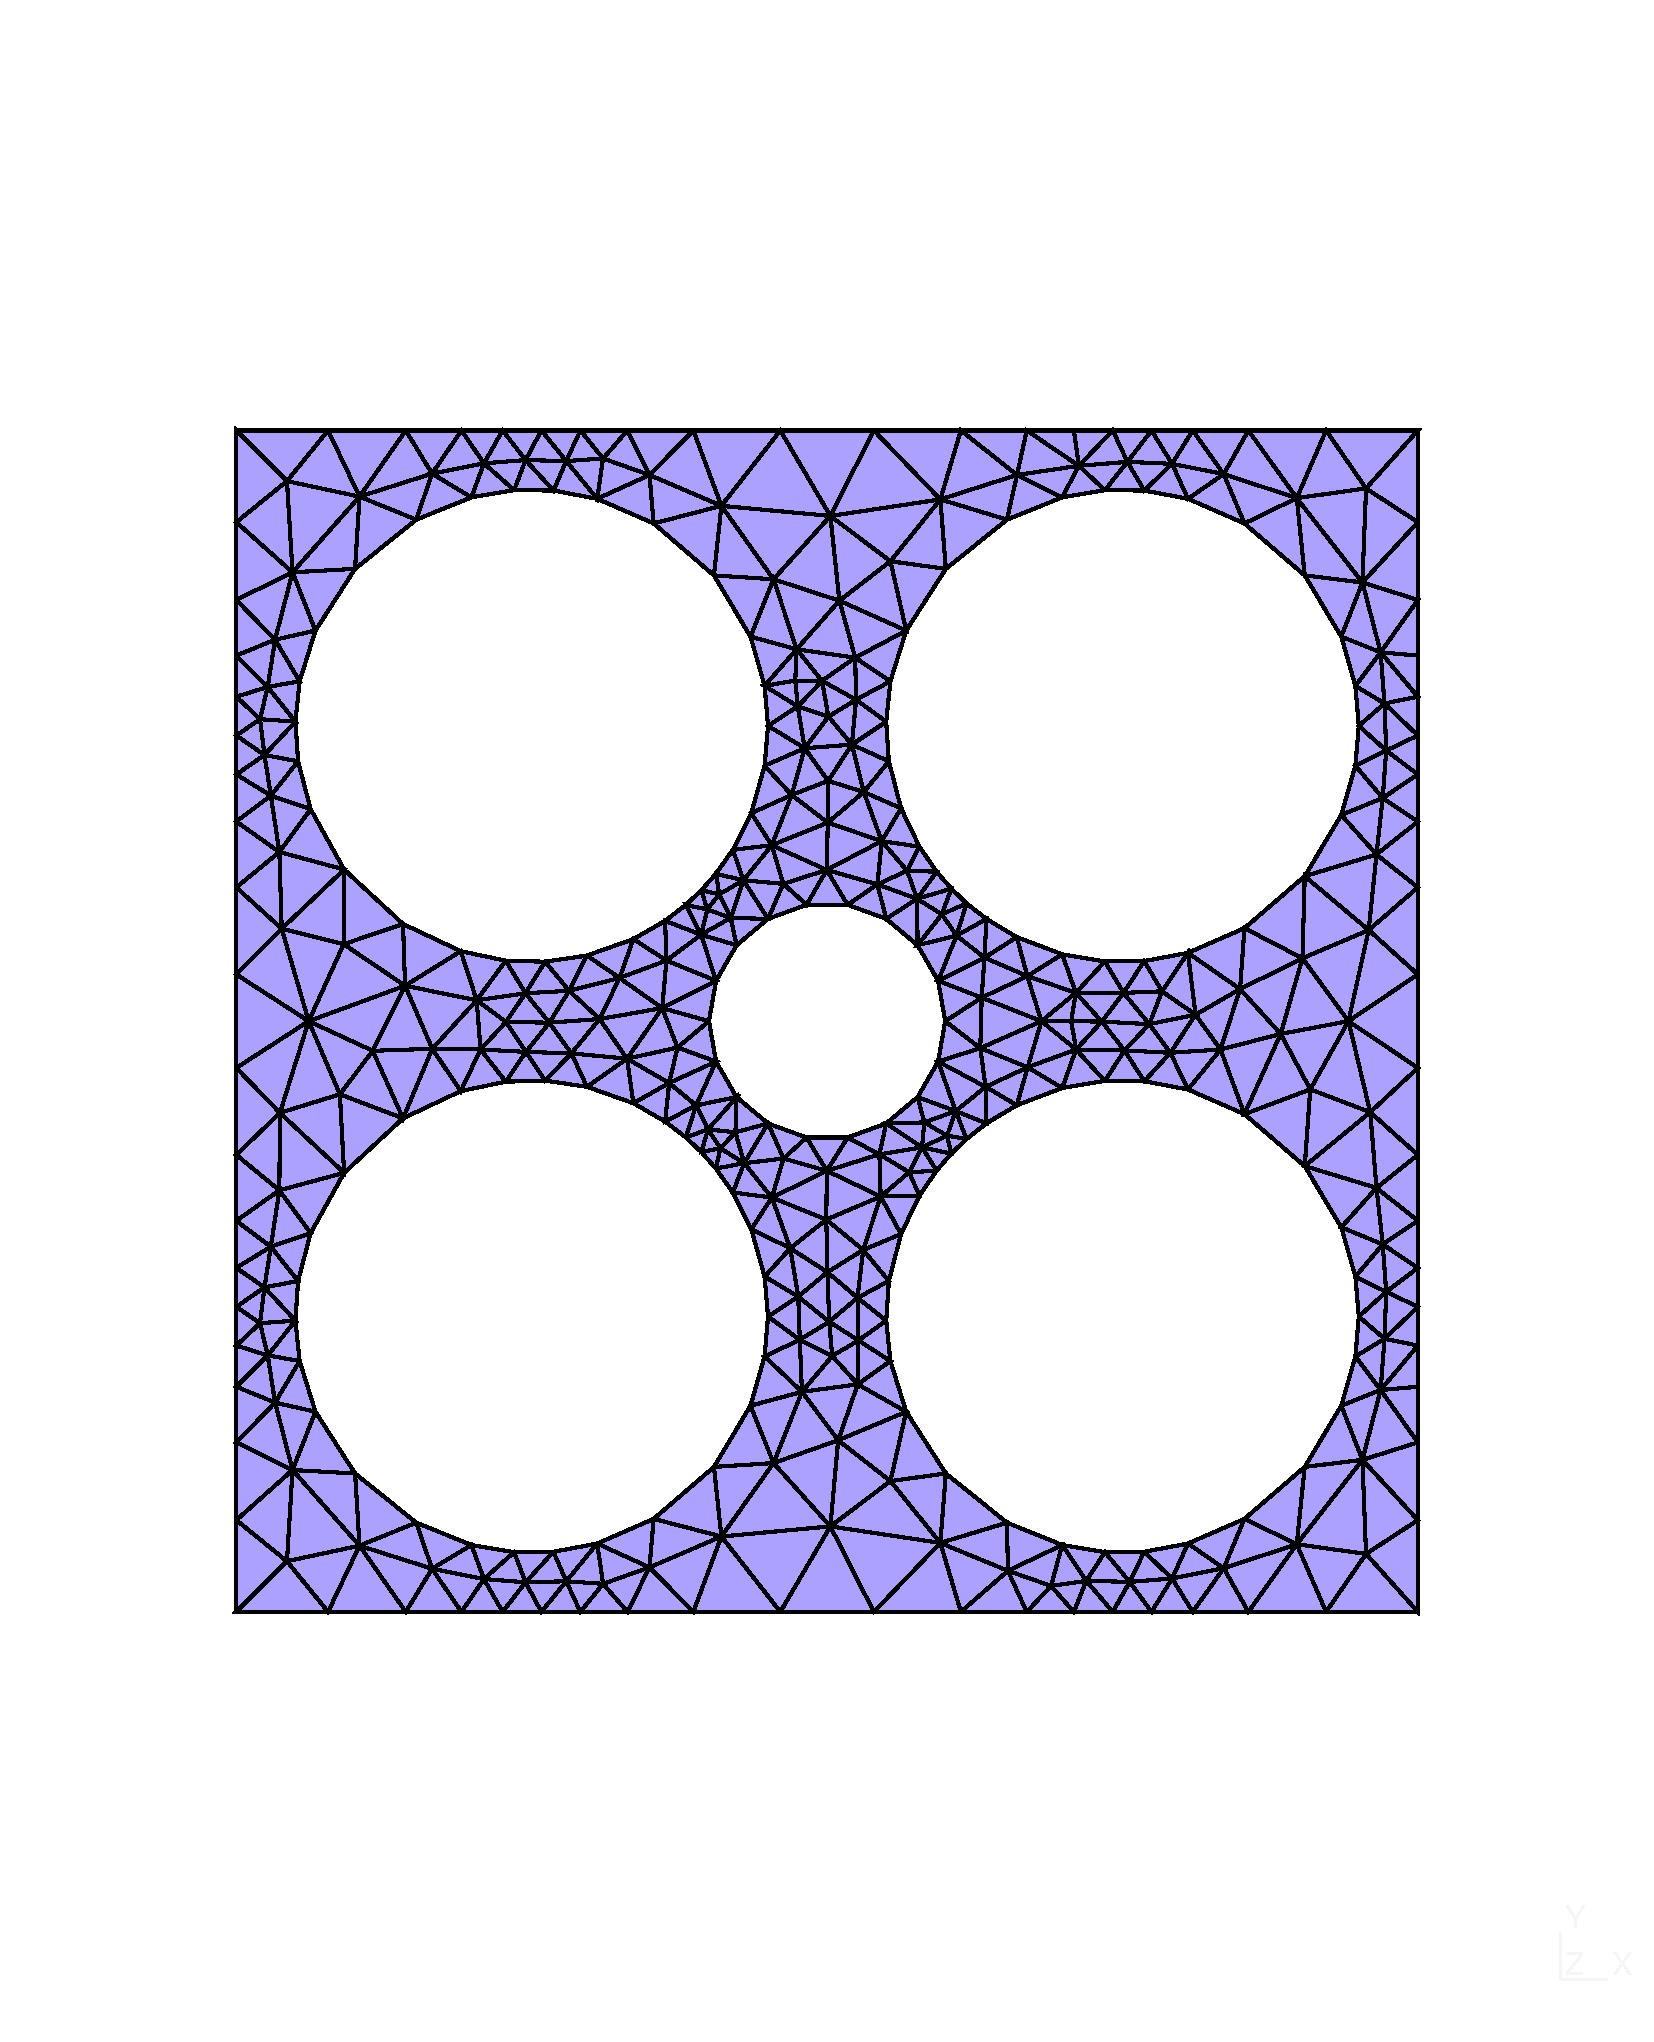
\includegraphics[width=\textwidth]{Figures_\version/tasks/5_star.pdf}
    \caption{Task 4}
    \label{fig:task4}
  \end{subfigure}
  \caption{Different domains introduced as different tasks.}
  \label{fig:tasks}
\end{figure}


\subsection{Results}\label{subsec:results}

\section{Discussion}\label{sec:discussion}

\section{Conclusion}\label{sec:conclusion}


%% \appendix

% To print the credit authorship contribution details
%\printcredits

%% Loading bibliography style file
%\bibliographystyle{model1-num-names}
\bibliographystyle{cas-model2-names}

% Loading bibliography database
\bibliography{/home/taylanot/Dropbox/archive_bib/aleksandr_colab.bib}

% Biography
%\bio{}
% Here goes the biography details.
%\endbio

%\bio{pic1}
% Here goes the biography details.
%\endbio

\end{document}

